Bei der Recherche zur allgemeinen Deflektometrie fällt auf, dass das Hauptforschungsgebiet der gegenwärtigen Deflektometrie die Generierung von dreidimensionalen Modellen von spiegelnden Objektoberflächen ist.
Der Aufbau eines solchen Anwendungsfalls sieht eine Beleuchtungseinheit (z. B. einen Bildschirm), ein Sensor (z. B. eine Kamera) und ein zu untersuchendes Objekt vor.

\begin{figure}[H]
	\centering
	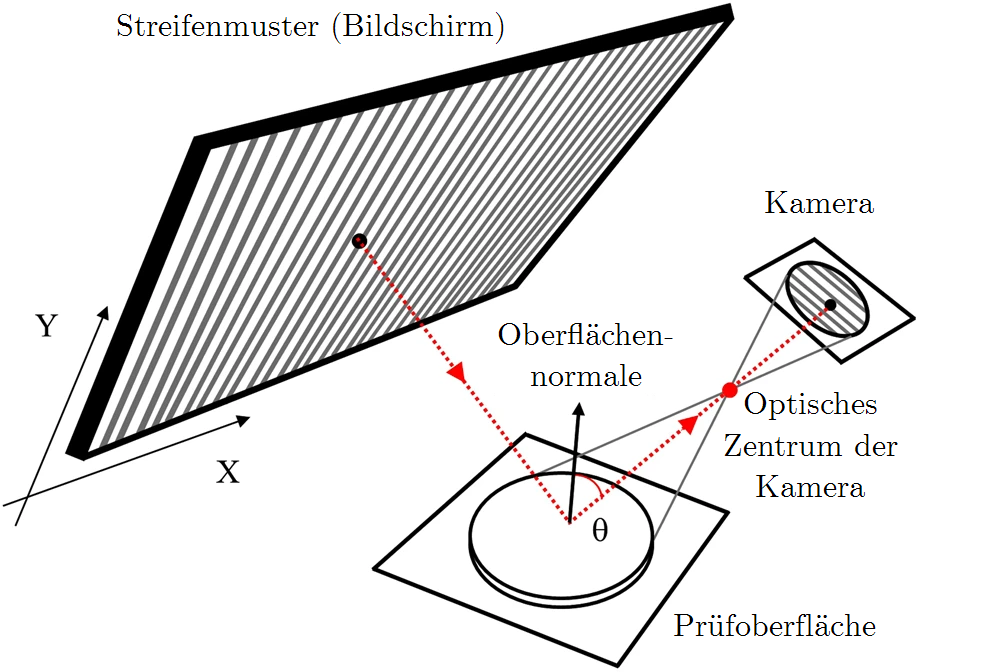
\includegraphics[width=0.8\textwidth]{02_grundlagenZurDeflektometrie/rekonstruktion/figures/nature-articel-nr1}
	\caption[Aufbau einer Deflektometrie-Prüfstation]{Aufbau einer Deflektometrie-Prüfstation. \textit{in Anlehnung an} \cite{aufbau}}
	\label{img:aufbau}
\end{figure}

\noindent
Wie in Abbildung \ref{img:aufbau} angedeutet, wird ein Muster auf ein Prüfobjekt projiziert und anschließend von einer Kamera aufgenommen.
Für dieses Verfahren werden zur Projektion üblicherweise Streifenmuster ge\-wählt, deren Grauwertverläufe in ihren Ausbreitungsrichtungen einer Sinus-Funktion entsprechen.
Das grundlegende Prinzip basiert darauf, dass jeder Punkt des Objekts dem richtigen Punkt auf dem Bildschirm zugeordnet wird.
Dabei ordnet man jedem Pixel des projizierten Musters, das man über die Kamera aufnimmt, sein zugehöriges Pixel des erzeugten Musters auf dem Bildschirm zu.
Der Vorteil bei sinusförmigen Streifenmustern ist, dass man für die Punkte des Objekts jeweils den Phasenwinkel im sinusförmigen Muster berechnen kann.
Dies erleichtert die Zuordnung von Kamera- und Bildschirmpunkten.
Durch diese Zuordnung von Kamera- und Bildschirmpunkten lassen sich Neigungsinformationen der Oberfläche berechnen.
Dies kann durch Strahlenverfolgungen erreicht werden.
In Abbildung \ref{img:aufbau} lässt sich das über die in Rot eingezeichneten Vektoren erkennen.

\p
Am Punkt des Auftreffens des Lichtstrahls auf das Objekt wird es auf eine bekannte Stelle in die Kamera reflektiert.
Nimmt man zusätzlich die Informationen über den Systemaufbau hinzu bzw. führt eine Systemkalibrierung durch, kann aus der Zuordnung von Kamera- und Bildschirmpunkten der Reflexionswinkel $\theta$ aus Abbildung \ref{img:aufbau} berechnet werden.
Da bei einer Reflexion die Lichtstrahlen genau an der Oberflächennormalen gespiegelt werden, lässt sich dann in einem weiteren Schritt die Oberflächennormale in diesem Punkt bestimmen.
Führt man dies für jeden Punkt im Kamerabild durch, erhält man daraus die Neigungsinformationen des zu prüfenden Objektes in der Form eines Normalenfelds.

\p
Schließlich ist es möglich, aus diesem Normalenfeld räumliche Information der Oberfläche zu berechnen.
Dafür kann man zunächst aus den Normalenvektoren die zugehörigen Tangentialebenen berechnen, die über je zwei Richtungsvektoren definiert sind.
Diese Richtungsvektoren bilden die Tangentialfelder des Prüfobjekts.
Man kann über eine Integration der Tangentialfelder in ausgewählte Richtungen Kurven bestimmen, die in der Oberfläche des Objekts liegen.
Durch diese Integration erhält man einen Höhenzusammen\-hang der Oberflächenpunkte.
Wenn zusätzlich ein Oberflächenpunkt gegeben ist, kann man die berechneten dreidimensionalen Positionen der Oberflächenpunkte im Raum angeben.\cite{kit_werling}